\documentclass[../thesis.tex]{subfiles}

\begin{document}

To reach into confined spaces robot arms must be thin, long, and maneuverable.
A thin robot may have small actuators with limited torque such that the joints cannot support the weight of the outstretched cantilevered arm.
However confined spaces are filled with places to rest for support, and contact forces can compensate for low joint torque. 
Robot motion planners that take advantage of support extend the reach and improve stability for long thin arms.

This chapter considers motion planning for a robot arm that may experience contact forces.
The motion planner's goal is to output a trajectory of joint positions that will move the robot from an initial configuration to a configuration with the end effector in a specified location.
This motion is achieved through actuators applying torques at these joints.
%% start with the robot arm in an initial configuration in joint space, and end with the end effector in a specified location.
Each joint can only apply a limited torque, and the trajectory must respect these limits.
The arm experiences forces due to gravity, inertial, friction, and also interaction with the environment, and this dynamics model is described in detail in section \ref{sec:robot_dynamics}.
Contact forces can be helpful by balancing out gravity, or detrimental by blocking a desired motion.
Contact forces prove difficult due to their large but local effect.


Section \ref{sec:trajectory_optimization} describes a solution to the motion planning task that uses trajectory optimization and is strongly based on Contact Invariant Optimization \cite{Mordatch2012}.
%% The problem formulation includes a function that assigns a cost to each trajectory, and uses the gradient of this cost function to incrementally improve the trajectory.
%% Typically a trajectory is penalized for large joint torques and for not reaching the goal, however that formulation provides insufficient gradient information when contacts are involved.
%% dynamics model is augmented, making it less accurate but better conditioned for optimization.
To better condition the problem for optimization, the dynamics are augmented to create smooth gradients around contacts.
Section \ref{sec:sample_planning} describes a sample-based planner capable of using contact forces, and again alterations are made to handle the thin contact manifold.







%% \section{Related Work}
\section{Robot Dynamics} \label{sec:robot_dynamics}

\begin{figure}
  \centering
  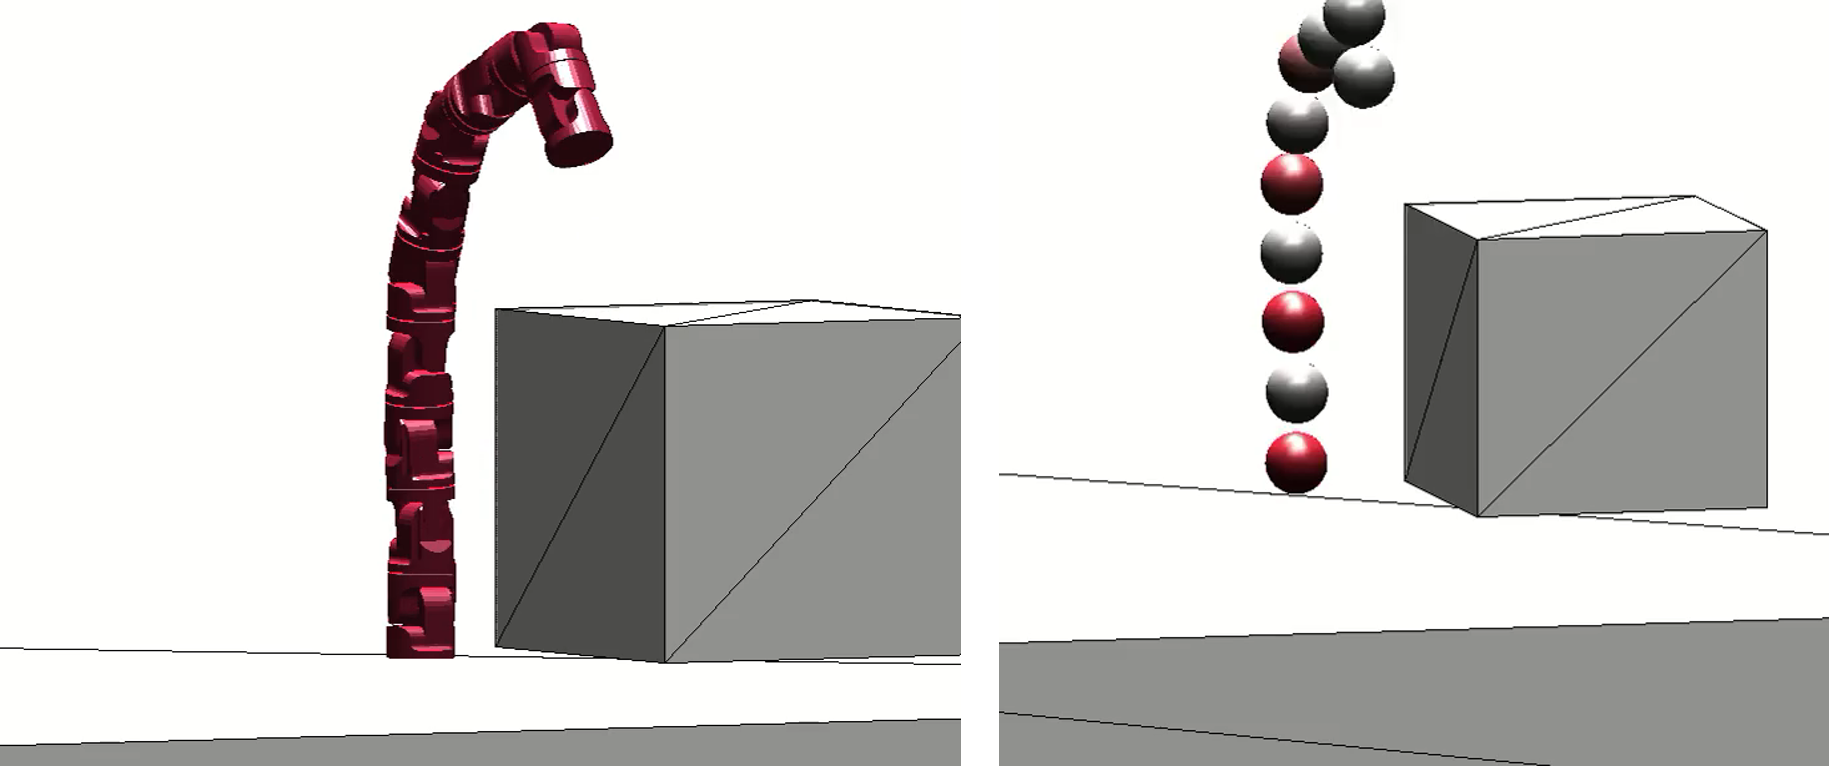
\includegraphics[width=.7\linewidth]{./Planning/sphere_approxmation.png}
  \caption{The visually accurate robot model (left) and the spherical approximation (right)}
  \label{fig:sphere_approximation}
\end{figure}


When not in contact with the environment the robot model follows the manipulator arm equation \cite{murray1994mathematical}:
\begin{align}
  M(\theta)\ddot \theta + C(\theta, \dot\theta)\dot\theta + N(\theta, \dot\theta) = \tau \label{eq:manipulator}
\end{align}
$M$ and $C$ are determined through the robot's known mass characteristics.
$N$ includes both gravity and frictional terms.
In practice $M, C,$ and $N$ do not need precise estimation, because closed loop controllers on the robot can compensate for errors.

\subsection{Accurate Contact Model}

Modeling the dynamics when the robot is in contact with the environment is significantly more challenging, and creating useful contact models is still an active area of research \cite{Posa2013}\cite{del2012control}\cite{Tonneau}.
This section describes a somewhat accurate contact model, however this model is ultimately not used in my path planning approahces.
The purpose of introducing this model is to illustrate the challenges of planning with accurate contact forces.

The true contact forces are caused by strain due to deformations in the environment and robot which are complicated to model accurately \cite{Saund2013}, so I make the following assumptions when modelling contact force as a function of joint angle.
\begin{enumerate}
\item Deformations of the environment obey a linear spring model, with spring constant k \cite{blandford2003applications}.
\item The robot arm has a discrete set of defined sections which may be in contact with the environment. In this work each section $i$ is modeled as a sphere with radius $r_i$, as shown in Figure \ref{fig:sphere_approximation}.
\item The robot arm is rigid.
\end{enumerate}\\



To calculate the contact force, first the deformation vector ${\bf d_i}$ of the environment is calculated for each contact section $i$ on the robot.
$d_i$ is the shortest vector in $R^3$ which translates sphere $i$ out of the penetration with the environment.
${\bf d_i}$ is ${\bf 0}$ if sphere $i$ does not intersect any object in the rigid environment.
%% ${\bf d_i}$ is the vector  sphere $i$ penetrates the rigid environment.
The contactact force felt by section $i$ is:
\begin{align}
  f_i = k {\bf d_i}.
\end{align}

Contact force $i$ adds to the joint torques dependant on the jacobian of section $i$ \cite{murray1994mathematical}:
\begin{align}
  \tau = J_{i}^T F_i
\end{align}



\subsubsection{Challenges with the Accurate Contact Model}
\begin{figure}
  \centering
  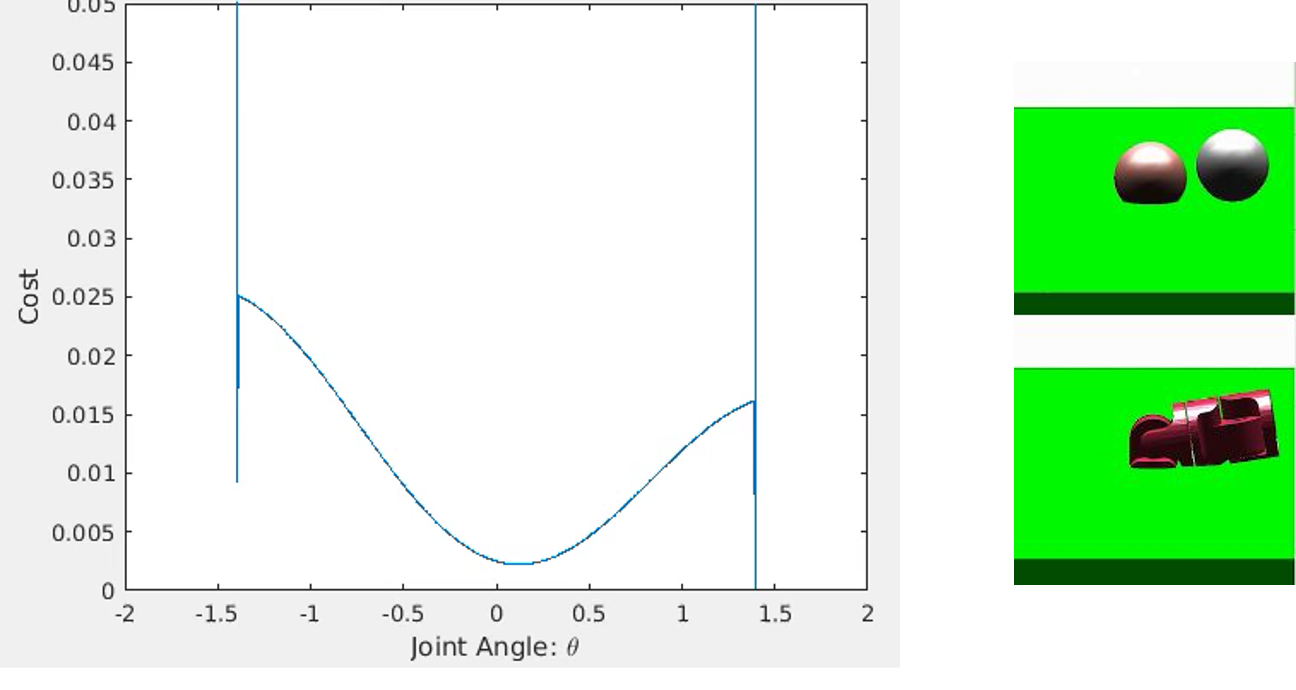
\includegraphics[width=\linewidth]{./Planning/naive_cost}
  \caption{Naive cost function, with sharp changes around contact locations}
  \label{fig:naive_cost}
\end{figure}

To illustrate the challenges with planning using an accurate contact model, consider the following toy problem.
A single configifuration is desired for a 1DOF robotic arm that minimizes a cost function which penalizes both torque and distance from a goal.
For specific implementation, a quadratic cost function is chosen:
\begin{align}
  L(s) = \sum ||\tau_{joint}||^2 + d^2
\end{align}


Figure \ref{fig:naive_cost} shows such a cost function, with the goal position at $\theta=1.4$.
At $\theta=0$ there is no cost due to torque, as the arm is balanced vertically, but there is cost due to not achieve the goal position.
At approximately $\theta= \pm 1.4$ the arm perfectly rests on the ground, so again there is no cost due to torque.
Moving slightly towards $\theta=0$ breaks the contact, so torque increases.
Moving slightly away from $\theta=0$ forces the arm further into the ground, drastically increasing the contact force and therefore joint torque.

The global minimum of this cost function, which indeed has the arm near the goal and also benefits from resting on the ground, is a narrow sliver, making this function poorly conditioned for optimization.
Iterative optimizers tend to fall into the wide basin of attraction for the local minima at $\theta=0.1$, as there is no guidance towards the global minima.
To find the global minima optimizers need to either evaluate the cost function for a huge number of states, get lucky, or have additional information to guide the search.
%% Nearly all initializations will result in convergence to the local minimum with the wide basin of attraction at $\theta=0.1$.
%% To effectively use trajectoy optimization for this task, this cost function is augmented to be better suited for optimization.




Although not perfect, the contact model described above has the correct structure.
There is no contact force when the arm is in free space, and the contact force increases quickly once the robot joints push the arm into the environment.
In this model, robot joint angles which cause significant penetration yeild huge joint torques, while in reality either the robot or environment would physically fail.
This discrepency is acceptable as both situations are not acceptable.
Since this structre is correct, attempting to make a more accurate contact model with not solve the problem.

%% first the smallest distance between each robot contact section and the environment is calculated, illustrated in Figure \ref{fig:contact_distance}.






%% The robot arm has defined sections which may be in contact with the environment.
%% For simplicity in calculations, these contact sections are approximated by spheres, shown in Figure \ref{fig:sphere_approximation}.
%% The environment is modeled as a triangular mesh, and contact occurs when a contact section intersects the mesh.
%% The contact force is determined by a spring model, and so the magnitude is proportional to the penetration distance, pushing the section out of the environment.
%% The physical robot and environment are both constructed of metal, so while a large spring constant provides a more accurate model this also causes numerical instabilities.
%% Each trajectory is simulated as a series of discrete time steps, and a large spring constant will result in giant forces for even the slight penetration this discretization introduces.

%% Figure \ref{fig:ThinManifold} illustrates the region of 

\subsection{Auxiliary Variables}
\begin{figure}
  \centering
  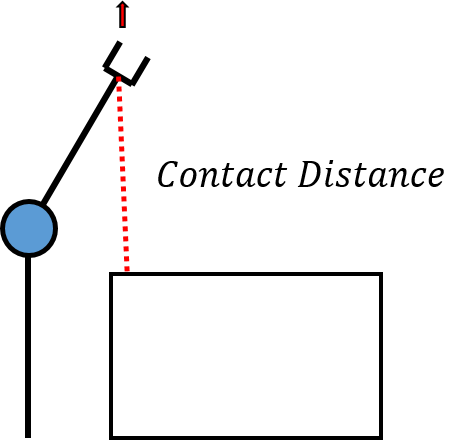
\includegraphics[width=.3\linewidth]{./Planning/contact_distance.png}
  \caption{Contact distance for the end effector section}
  \label{fig:contact_distance}
\end{figure}

\begin{figure}
  \centering
  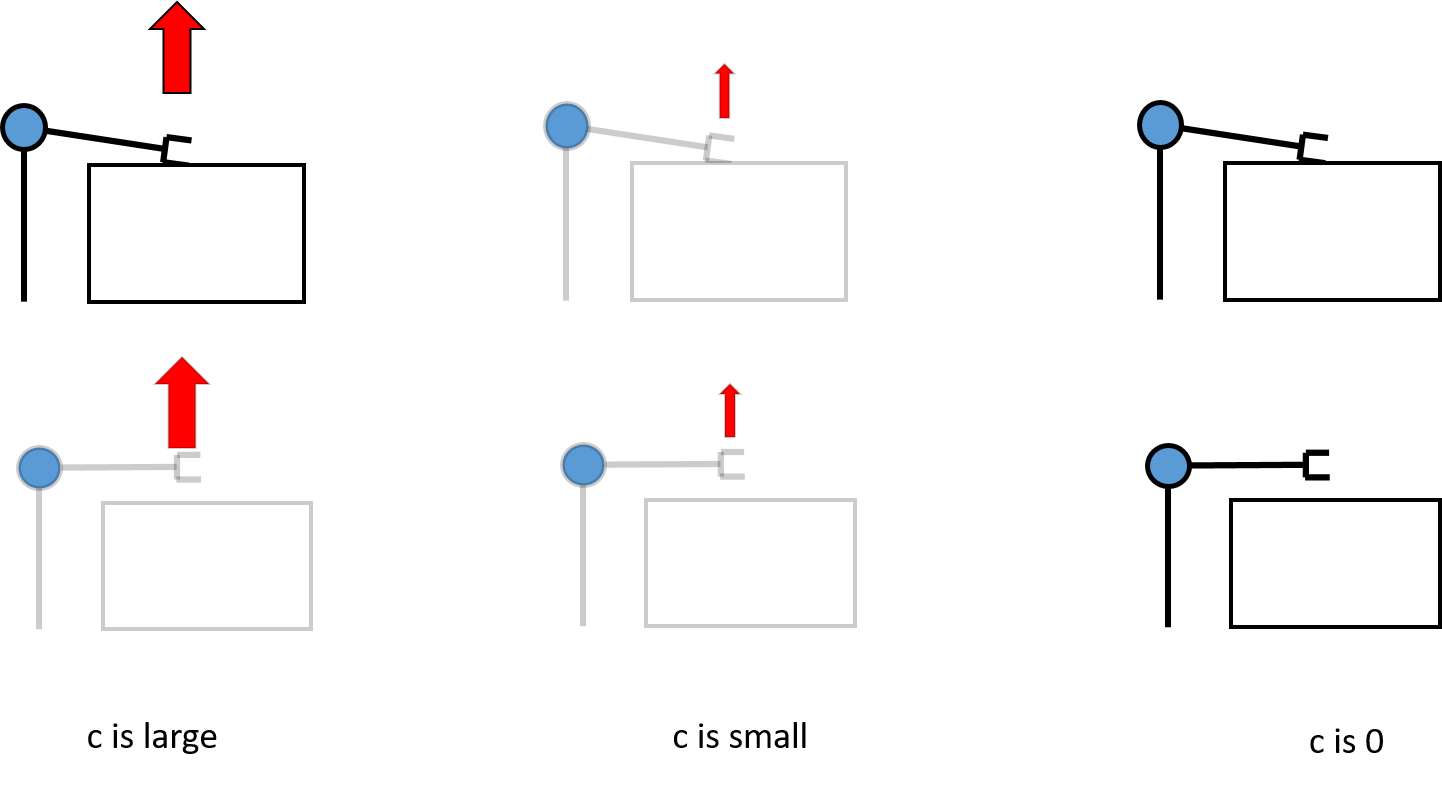
\includegraphics[width=.7\linewidth]{./Planning/ContactArms.png}
  \caption{Arm configuration and simulated (not realistic) contact forces for a variety of arm configurations and continuous contact variables}
  \label{fig:ContactArms}
\end{figure}


The key approach used in this work softens contacts through the introduction of auxiliary variables, which drastically smooth the cost function at the expense of increasing the dimensionality of the state space, using the approaches of Contact Invariant Optimization \cite{Mordatch2012}.
Appended to each state $s_t$ is a set of auxiliary continuous variables $c_t$, one for each section of the robotic arm allowed to make contact with the environment.
This augmented contact model no longer attempts to match reality, and allows for contact forces at a distance.
The variables $c_t$ regulate the magnitude of the normal and frictional artificial contact forces and will be described mathematically in section \ref{sec:smoothing}.
Robot states, as well as the input to cost functions, now include both the joint angles as well as the auxillary variables, and planners must plan for both simultaneously.

Figure \ref{fig:ContactArms} helps give intuition on how the contact variables influence these artificial contact forces.
In this figure the end effector is the only section allowed to make contact, and thus there is a single $c$.
Larger values for $c$ allow larger artificial contact forces to support the cantilevered arm.
The transparent configurations are physically infeasible, as in reality contact forces cannot be applied at a distance.
$c$ does not represent actual contact, but more closely represents the ``desire'' to add a contact.




%% These $c$ variables seem unnecessary as the forward kinematics specified by the joint angles $\theta$ determine the locations of the robot, and therefore determine the contacts between the robot and the environment.
%% Without this augmentations, slight changes in these joint configurations result in slight motion of the robot which may result in huge changes in contact forces.
%% Additionally without artificial terms in the cost function to model contact, the cost function is blind to potential contacts that may be close and useful.







\section{Trajectory Optimization} \label{sec:trajectory_optimization}

%% \begin{figure}
%%   \centering
%%   \begin{subfigure}[b]{0.24\linewidth}
%%     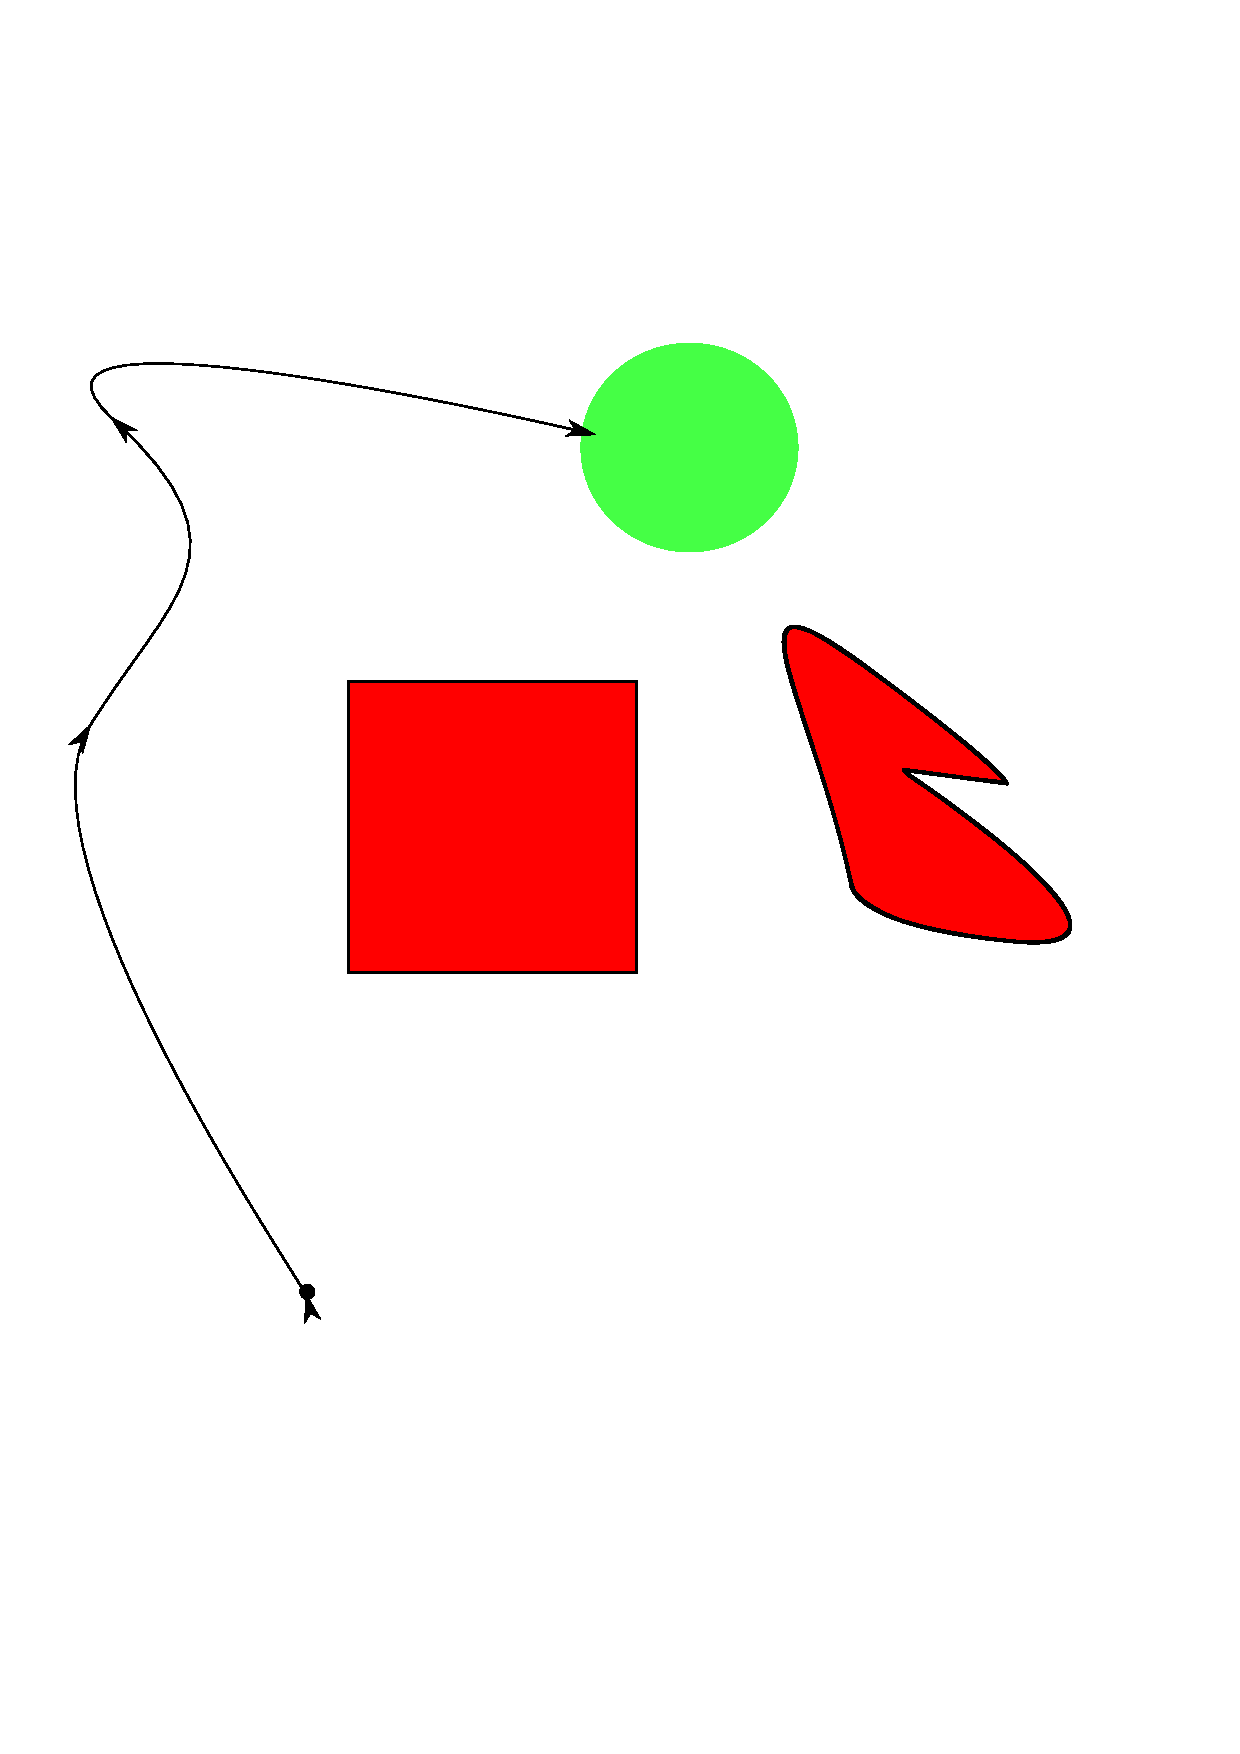
\includegraphics[width=\linewidth]{./Planning/trajectory_1.pdf}
%%   \end{subfigure}
%%   \hfill
%%   \begin{subfigure}[b]{0.24\linewidth}
%%     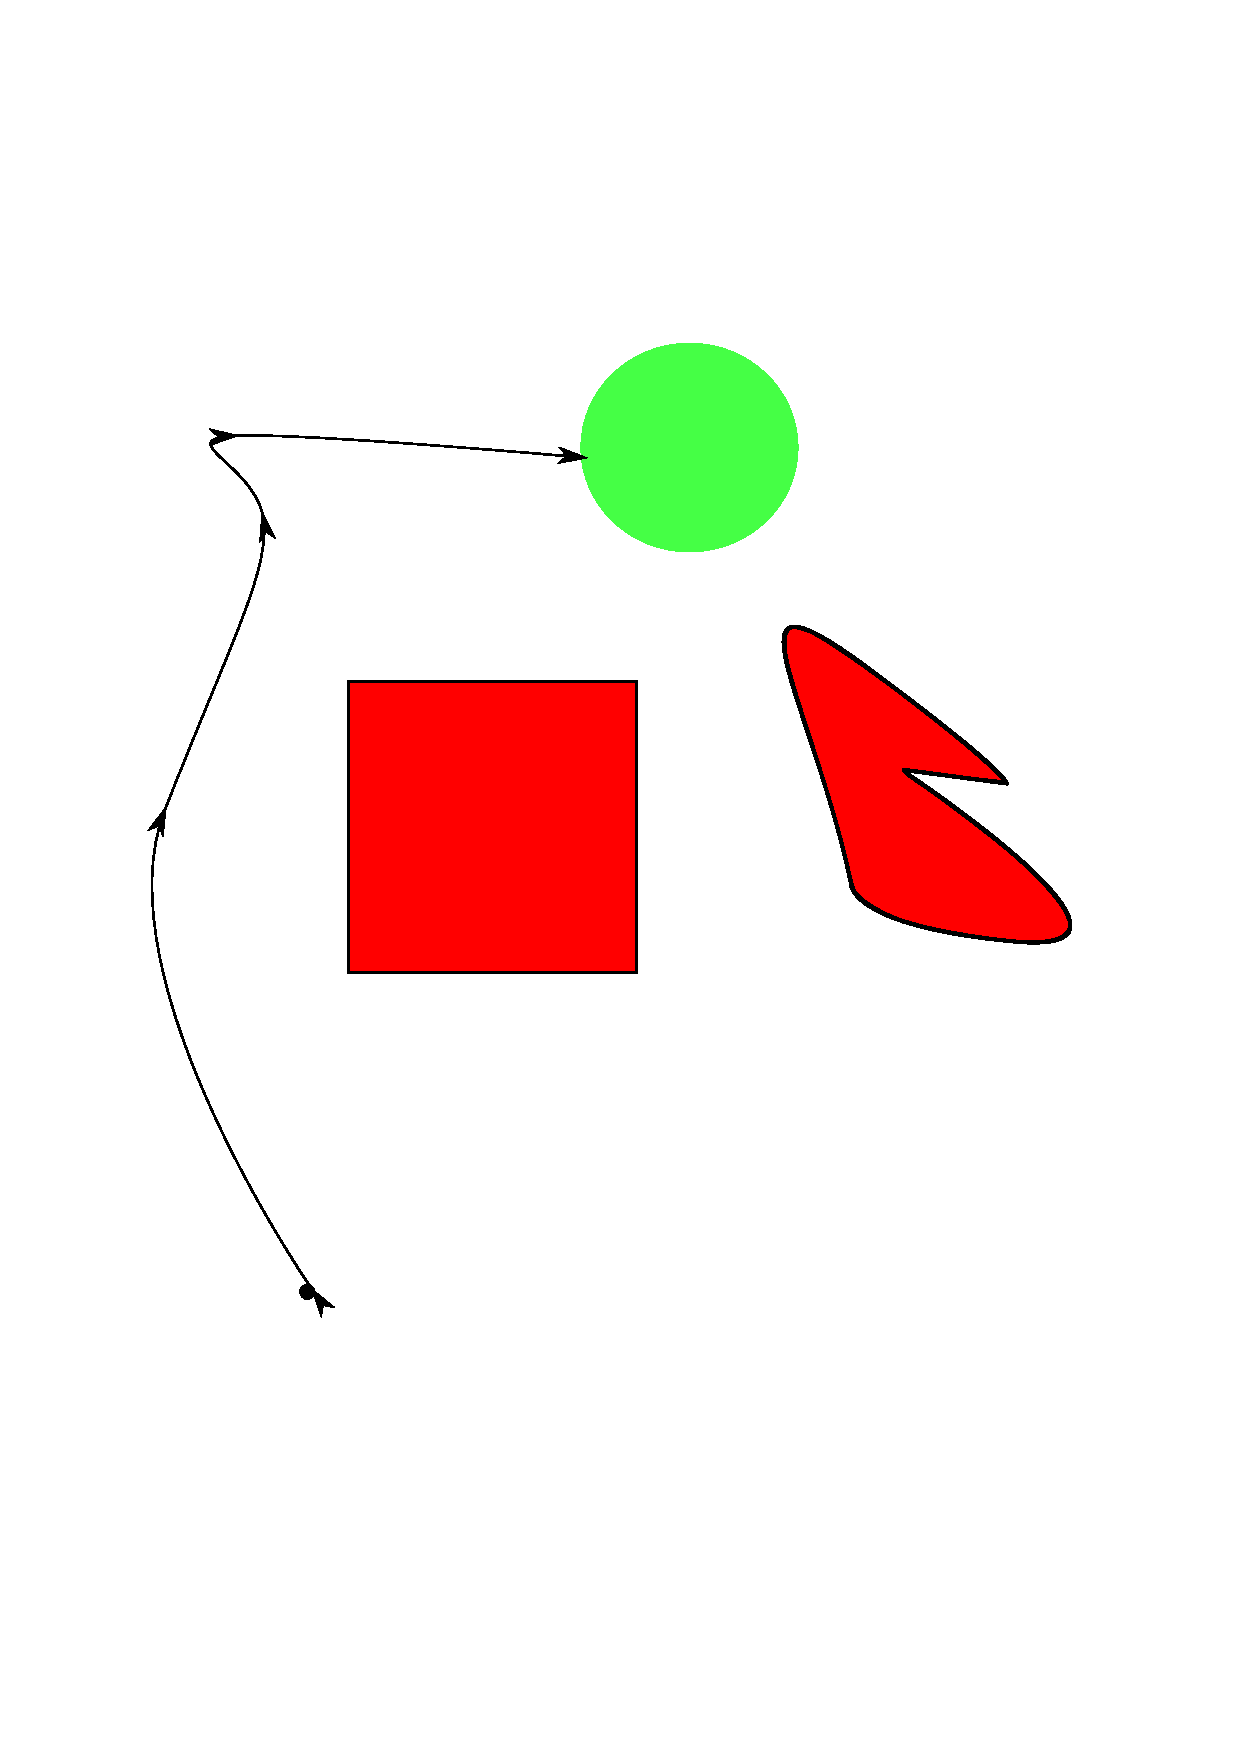
\includegraphics[width=\linewidth]{./Planning/trajectory_2.pdf}    
%%   \end{subfigure}
%%   \begin{subfigure}[b]{0.24\linewidth}
%%     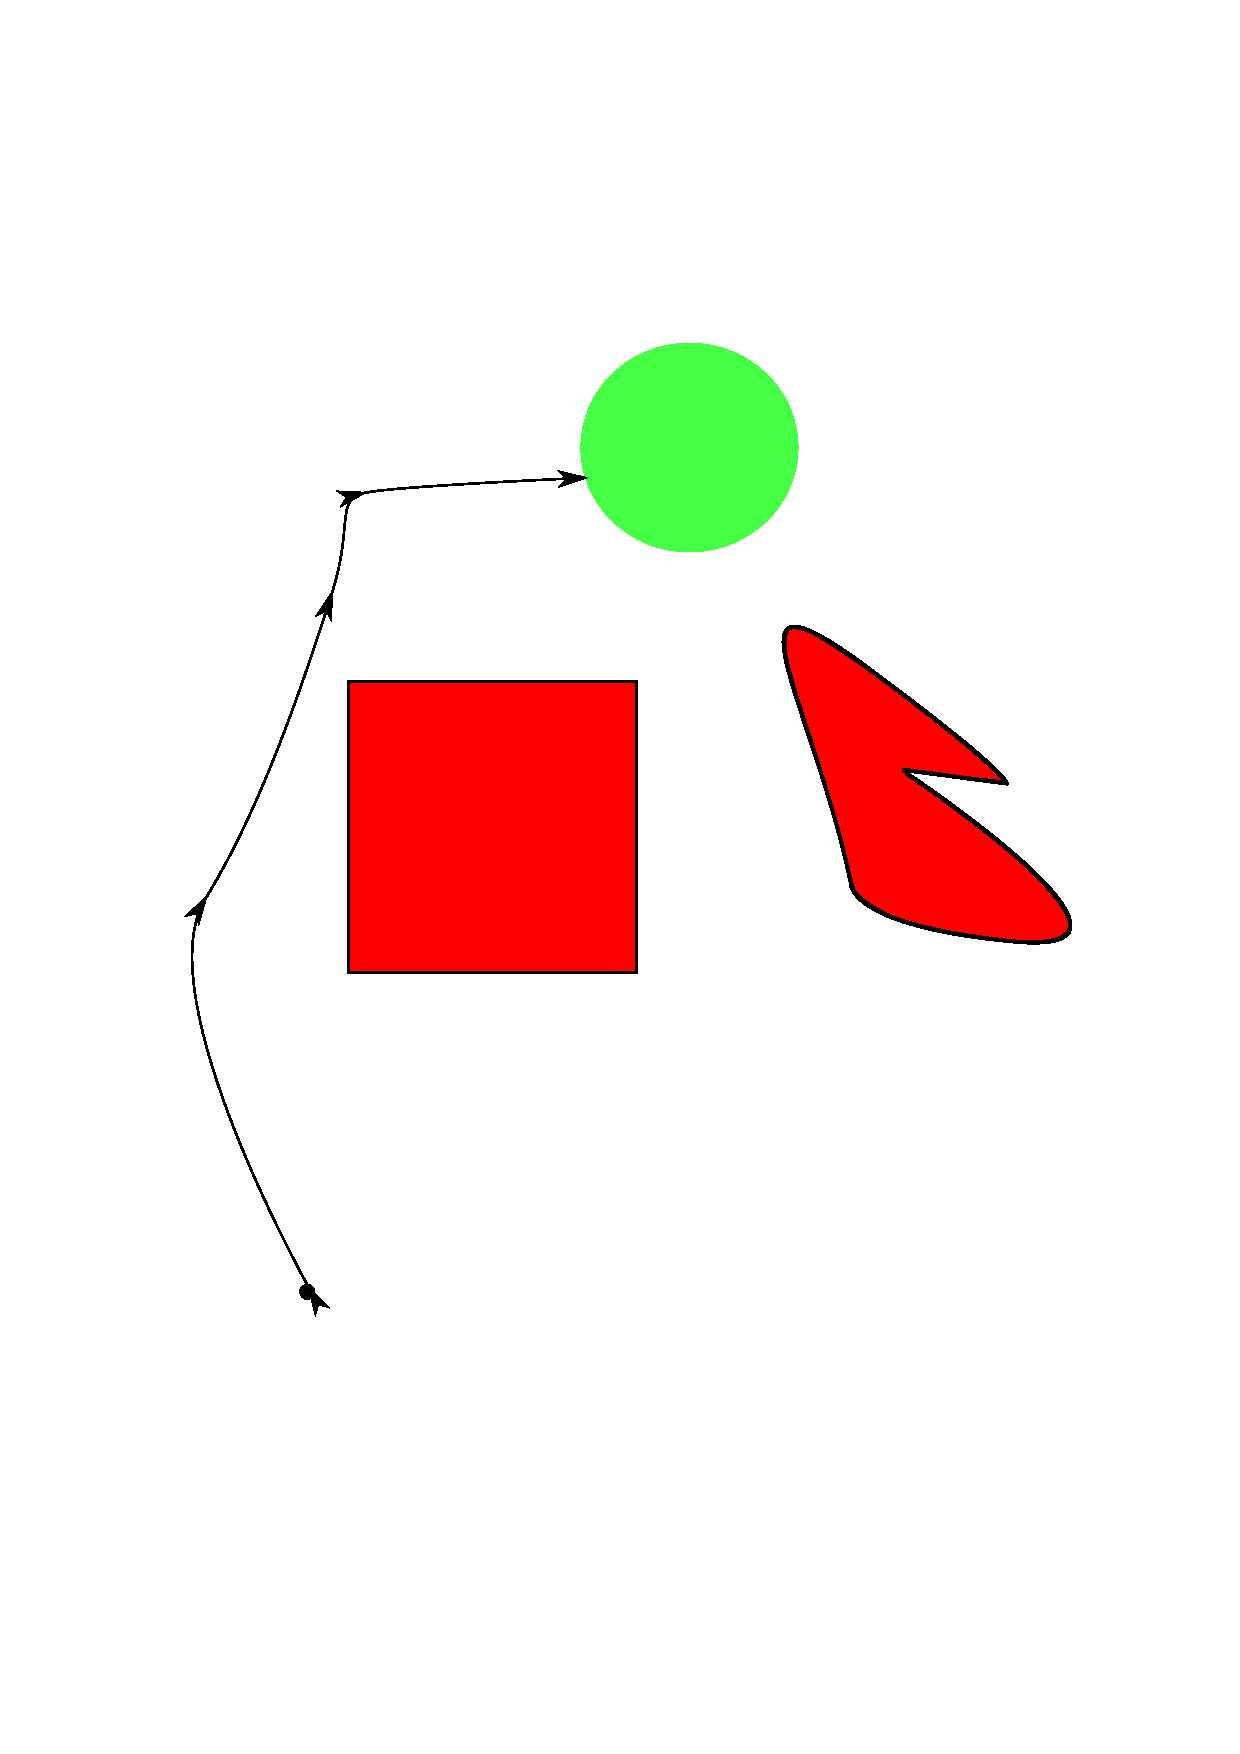
\includegraphics[width=\linewidth]{./Planning/trajectory_3.pdf}
%%   \end{subfigure}
%%   \hfill
%%   \begin{subfigure}[b]{0.24\linewidth}
%%     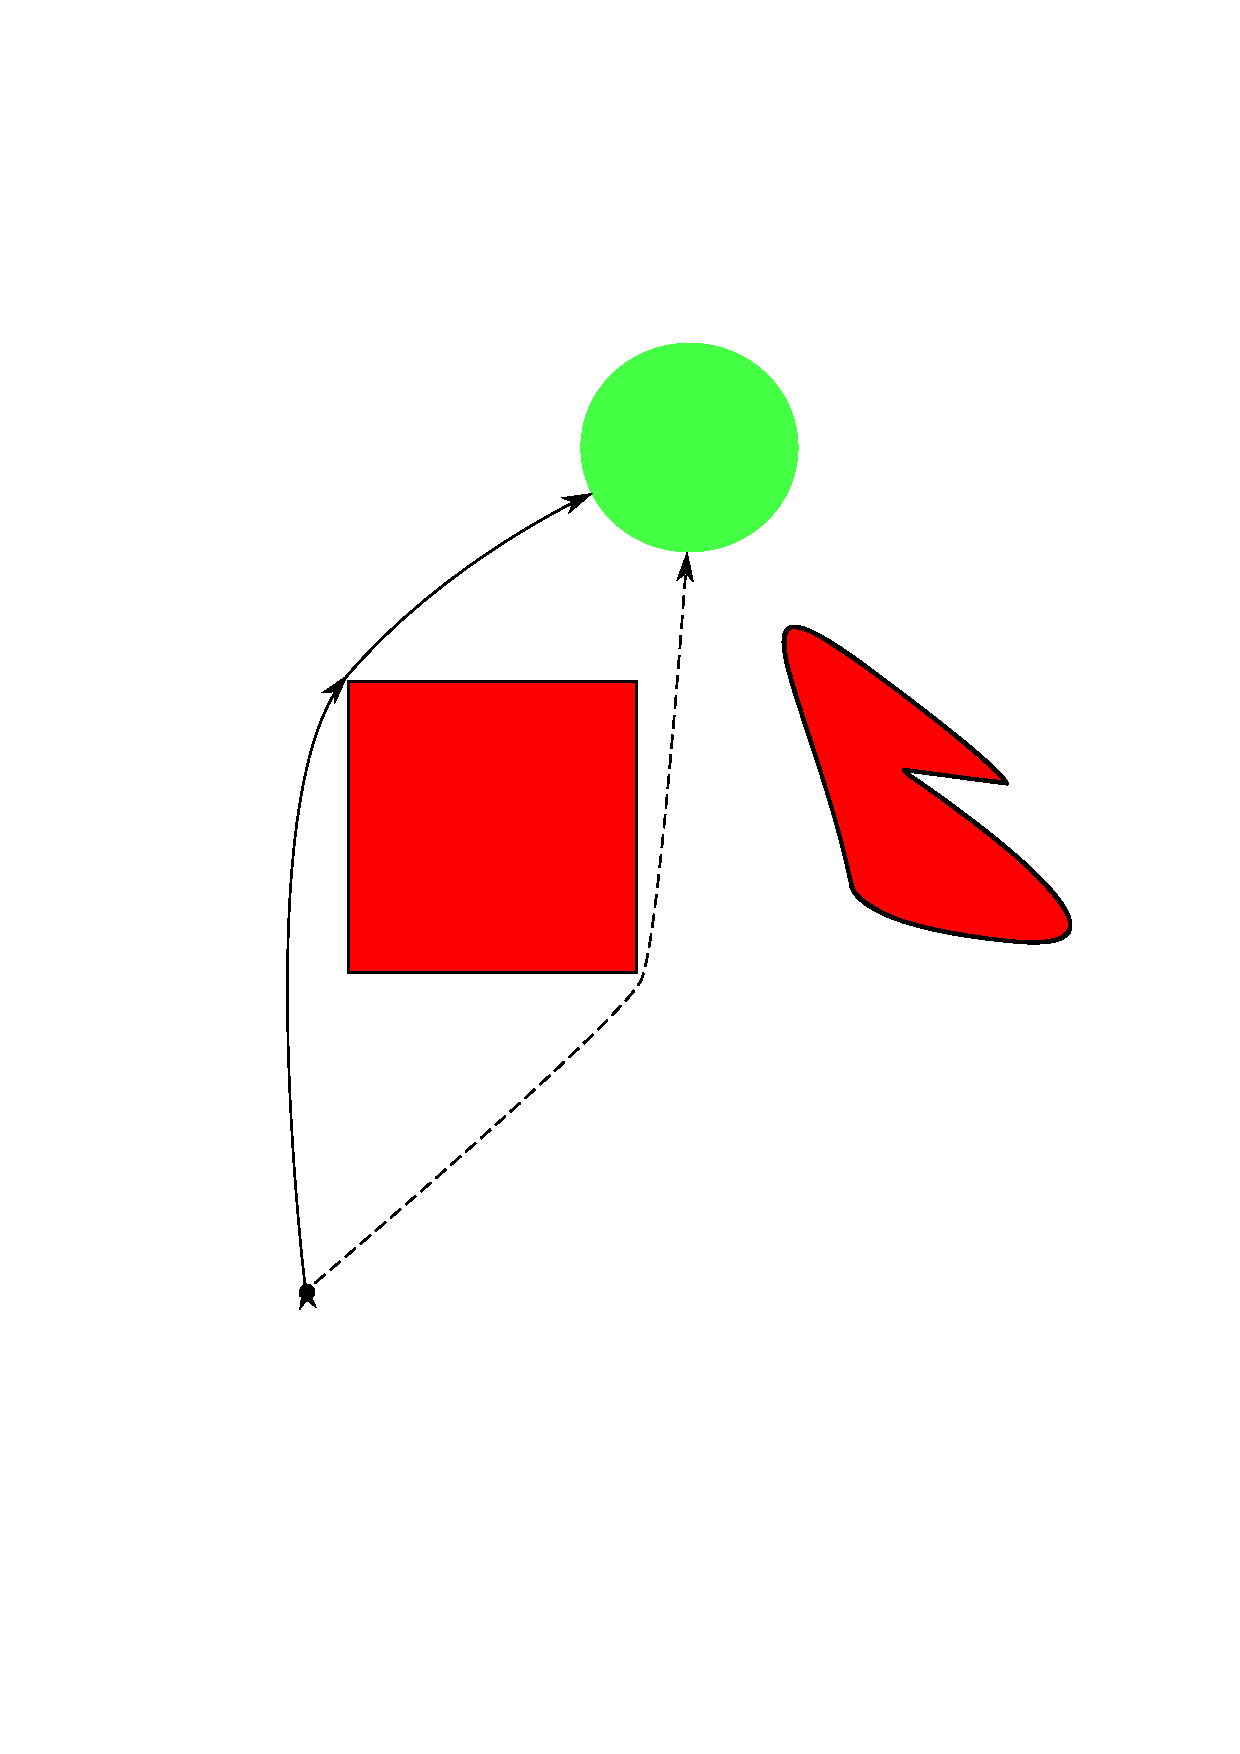
\includegraphics[width=\linewidth]{./Planning/trajectory_best.pdf}    
%%   \end{subfigure}
  
%%   \caption{Optimizing the shortest path trajectory from an initial path converges to a local best, but possibly misses the globally best solution.}
%%   \label{fig:TrajectoryOptimization}
%% \end{figure}


Trajectories for a robotic arm can be created through trajectory optimization, a process that progressively improves the cost of a trajectory.
In this work a trajectory $s$ is a discrete list of robot states $s_t$ at increasing points in time, where the state contains joint angles and perhaps auxillary variables.
To transition between timesteps, joint torques are calculated through inverse dynamics, and these torques must remain below the actuator torque limit.



%% The formulation used in the paper follows from Mordatch's work \cite{Mordatch2012}.







\subsection{Smoothing the Cost Function} \label{sec:smoothing}
A local optimal trajectory $s^*$ is computed by minimizing the cost function of the form

\begin{align}
L(s) &= L_{Object Penetration} + L_{Goal} \nonumber \\
&+   L_{Contact Violation} + L_{u}  \label{eq:cost}
\end{align}
    
$L_{Object Penetration}$ and $L_{Goal}$ are straightforward, while the interplay between $L_{Contact Violation}$ and $L_u$ provide the interesting structure allowing the optimization to find paths which use supporting contacts.




\subsubsection{Cost $L_{Contact Violation}$}
Each section $i$ of the robot able to make contact has an associated variable $c_{t,i} > 0$ at each time step. $c$ intuitively represents the allowable strength of the artificial contact force, which in the augmented dynamics model may occur even without physical contact.
%% Since if the robot is not physically in contact with the world there will not be a contact force the cost $L_{Contact Violation}$ is introduced to penalize non-zero values of $c$ when the robot is not in contact.
$L_{Contact Violation}$ places a penalty on forces applied at a distance to encourage physically real behavior.

For each robot section $i$, and each time step $t$:
\begin{align}
  L_{Contact Violation} = \gamma_{CV} \sum_t{\sum_{i\in sections}{c_{t,i} d_{t,i}}}
\end{align}

Figure \ref{fig:contact_distance} shows the contact distance $d$ for a section of a robotic arm. Since this distance is substantial, the magnitude of the associated contact variable will determine the contribution to cost. 
Non-zero values for $c$ are intentionally allowed when the robot is not in contact with the environment even though this is not physically realistic.
However, during optimizing either $c_{t,i}$ or $d_{t,i}$ will tend towards 0.
The term $\gamma_{CV}$ weights the cost of contact violation relative to other costs.
To ensure physically reallistic trajectories, this hyperparameter is increased as optimization progresses.







\subsubsection{Cost $L_u$}

\begin{figure}
  \centering
  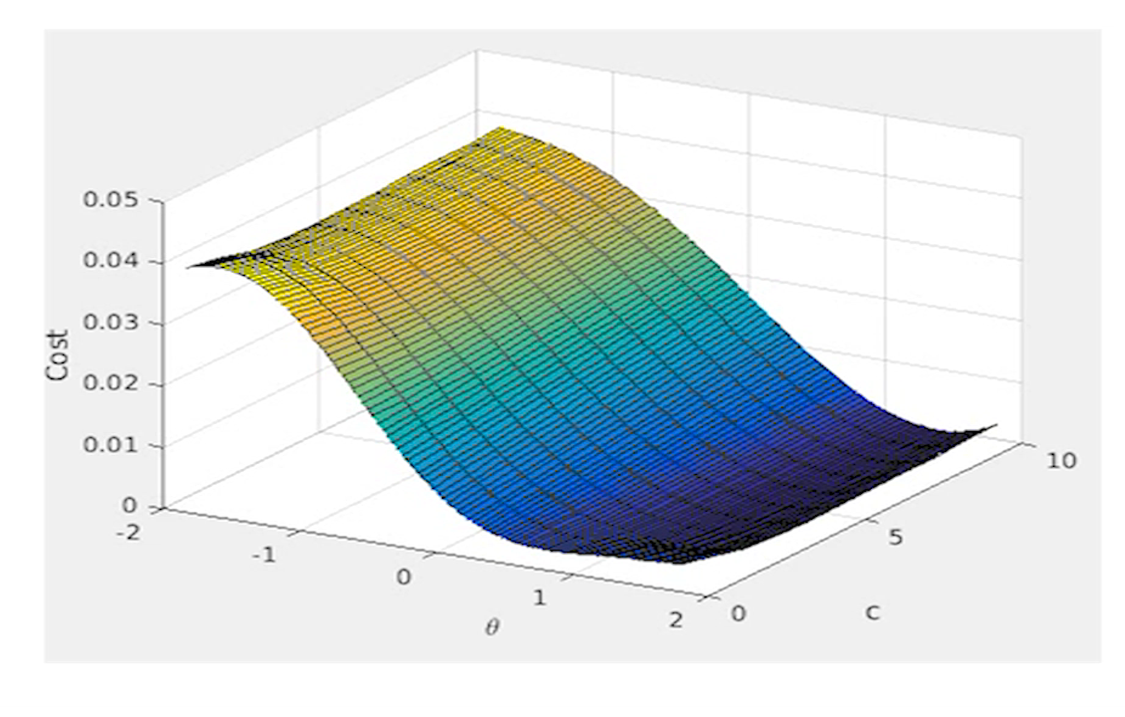
\includegraphics[width=.7\linewidth]{./Planning/augmented_cost.png}
  \caption{The cost function for the arm in Figure \ref{fig:naive_cost}, augmented with the auxiallary contact variable}
  \label{fig:augmented_cost}
\end{figure}


The cost $L_u$ penalizes the input torque, $u$,  necessary to follow the trajectory specified.
%% With no contacts these inputs could be calculated directly from the arm inverse dynamics.
%% As discussed the physical contact forces are extremely sensitive to robot configuration, so to soften the forces we instead compute the contact forces that minimize the joint torque.
%% When the trajectory is executed on the robot the joint controller will take responsibility for finding the slight adjustments in configuration to reach the desired contact forces.
%% The path planner does not have to worry about the minute adjustments for a model that will not match reality to that detail anyway.
%% Instead this path planner just needs to estimate the best contact forces possibly, according to the the following quadratic programming problem:
The contribution from the free manipulator, $\tau_{Free}$, is determined from the joint angles by Eq. \ref{eq:manipulator}.
The contribution from contact forces is not yet determined, since under the augmented dynamics model artificial contact forces can be applied even without physical contact.
Thus, these artificial contact forces are chosen optimistically to minimize the required joint torque, subject to regularization. 


\begin{align}
f, u &= argmin_{\tilde{f}, \tilde{u}} ||J^T\tilde{f} + \tilde{u} - \tau_{Free}|| \\
&+ \tilde{f}^T W \tilde{f} + \tilde{u}^T R \tilde{u}
\end{align}

The input control regularization $R$ is chosen based on the desired penalization of joint inputs. The contact force regularization $W$ is dependent on the values of $c$, with 
$$W_{j,j} = \frac{1}{c_{i,t}^2 + 1}$$
If $c$ is large then, the force regularization is small, so the contact force can be large.
If $c$ is small, the force regularization is large, thus the contact force is heavily penalized and will be small.

Figure \ref{fig:ContactArms} shows a robot arm in a variety of configurations and with several values of contact variables.
The red arrows indicate the simulated contact force.
If the contact variable is large, a large force can be applied to reduce joint torques even when there is no physical contact.
This serves to reduce the cost due to joint torques.
The competing cost $L_{Contact Violation}$ prevents this contact variable from growing too large for infeasible contacts.


Figure \ref{fig:augmented_cost} shows this augmented cost function for the arm in Figure \ref{fig:naive_cost}.
The dimensionallity of this cost function has increased, yet now there is a strictly descending path from the local minima of the naive cost function, $\theta=0.1$, to the global minima.
The basin of attraction for the global minima has increased dramatically.




\subsubsection{Other Cost Terms}
$L_{Obstacle}$ penalizes penetration of the robot into the environment which is calculated using the robot forward kinematics.
For simplicity, the same simplified spherical model is resued here.
This addition is necessary since the artificial contact model created by $L_u$ and $L_{ContactViolation}$ no longer ensures obstacle penetration produces high joint torques.

\begin{align}
  L_{Obstacle} = \sum d_{ObstaclePenetration}
\end{align}

$L_{Goal}$ is a penalty on the distance from the robot end effector at the last state $s_T$ to the goal location.
Since in this formulation reaching the goal is a soft constraint, the hyperparameter $\gamma_2$ can be adjusted to balance reaching the goal with applying joint torque.
\begin{align}
  L_{Goal} = \gamma_2 ||EndEffector_T - goal||
\end{align}


\subsection{Initialization Challenges}
Although the cost function augmentation described above greatly improves the conditioning of the cost function with respect to contacts, in practical problems this cost function is still plagued with local minima.
As a simple example, consider the situation in Figure \ref{fig:local_min}, where most initial trajectories will result in the arm never reaching the goal ``X''.

Straightfoward initialization techniques include random initialization with random restarts, and linear joint angle interpolation between starting configuration and a configuration that achieves the goal.
These initializations work well in open environments, but poorly in confined spaces.
Thus a sample based planner is employed to provide a diversity of good initializations.

\begin{figure}
  \centering
  \begin{subfigure}[b]{0.4\linewidth}
    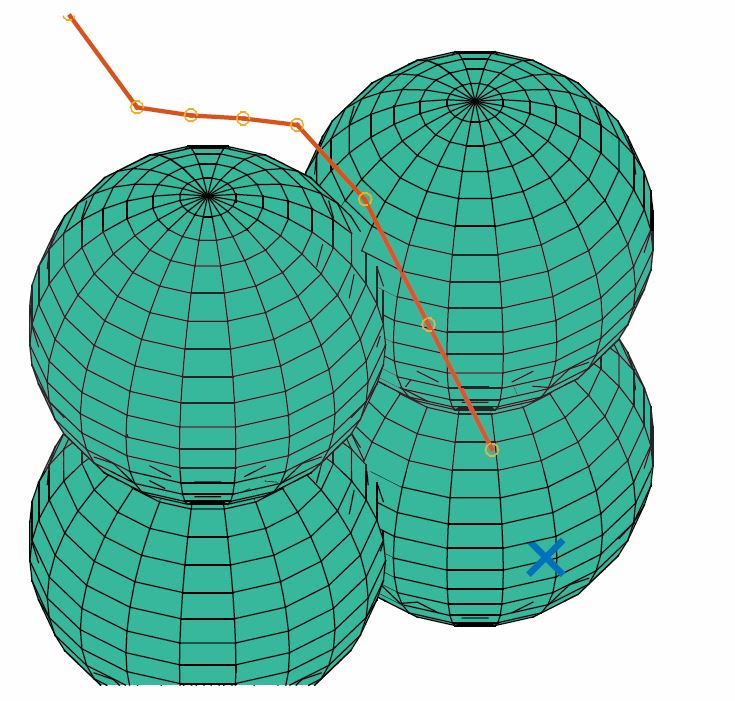
\includegraphics[width=\linewidth]{./Planning/Local.jpg}    
  \end{subfigure}
  \begin{subfigure}[b]{0.4\linewidth}
    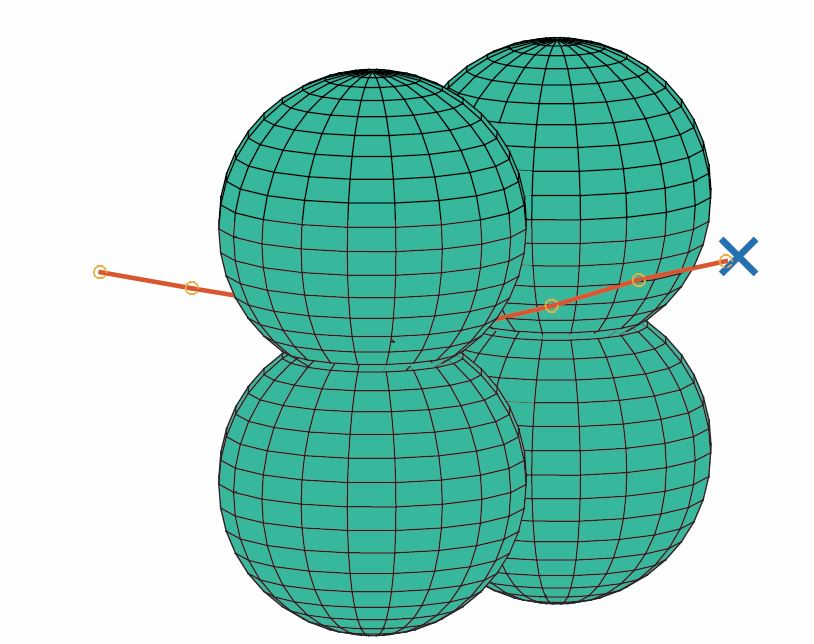
\includegraphics[width=\linewidth]{./Planning/global.jpg}    
  \end{subfigure}
  \caption{Trajectory optimization finding a local minimum (left) and the global minimum (right) for an arm attempting to reach the blue ``X''}
  \label{fig:local_min}
\end{figure}








\section{Sample Based Planning} \label{sec:sample_planning}
%% \subsection{RRTs and their variants}
It is possible to solve planning problems using a sample based planner, but once again the thin contact manifold causes challenges.
Sample based planners probabilistically sample configurations to explore the feasible space, and through sufficent exploration seek to find the trajectories to a goal while obeying constraints.
Specifically, this section employs the RRT, described in Algorithm \ref{alg:RRT}.
The basic RRT algorithm maintains a tree of trajectories (edges) to configurations (nodes), and grows this tree by ending to randomly sampled configuration.
As discussed in Section \ref{sec:related:RRT}, the basic linear extension fails when the only allowable space for the trajectory to grow is a thin manifold, as in the case of a supporting contact.

Figure \ref{fig:thin_manifold} illustrates this contact manifold.
In this example, in some regions of configuration space a contact is not needed to support the arm, and trajectories may progress in any direction.
The thin ribbon shows the manifold in configuration space where the arm makes contact with the environment. In the left region the contact is not needed and a trajectory is free to break the contact, however, the arm is able to reach the right region only by using the support of a contact force.
In cases where the configuration must remain on this manifold, linearly extending towards a randomly sampled point will quickly cause the trajectory to leave the manifold, and make little progress in extending the tree.



\begin{figure}
  \centering
  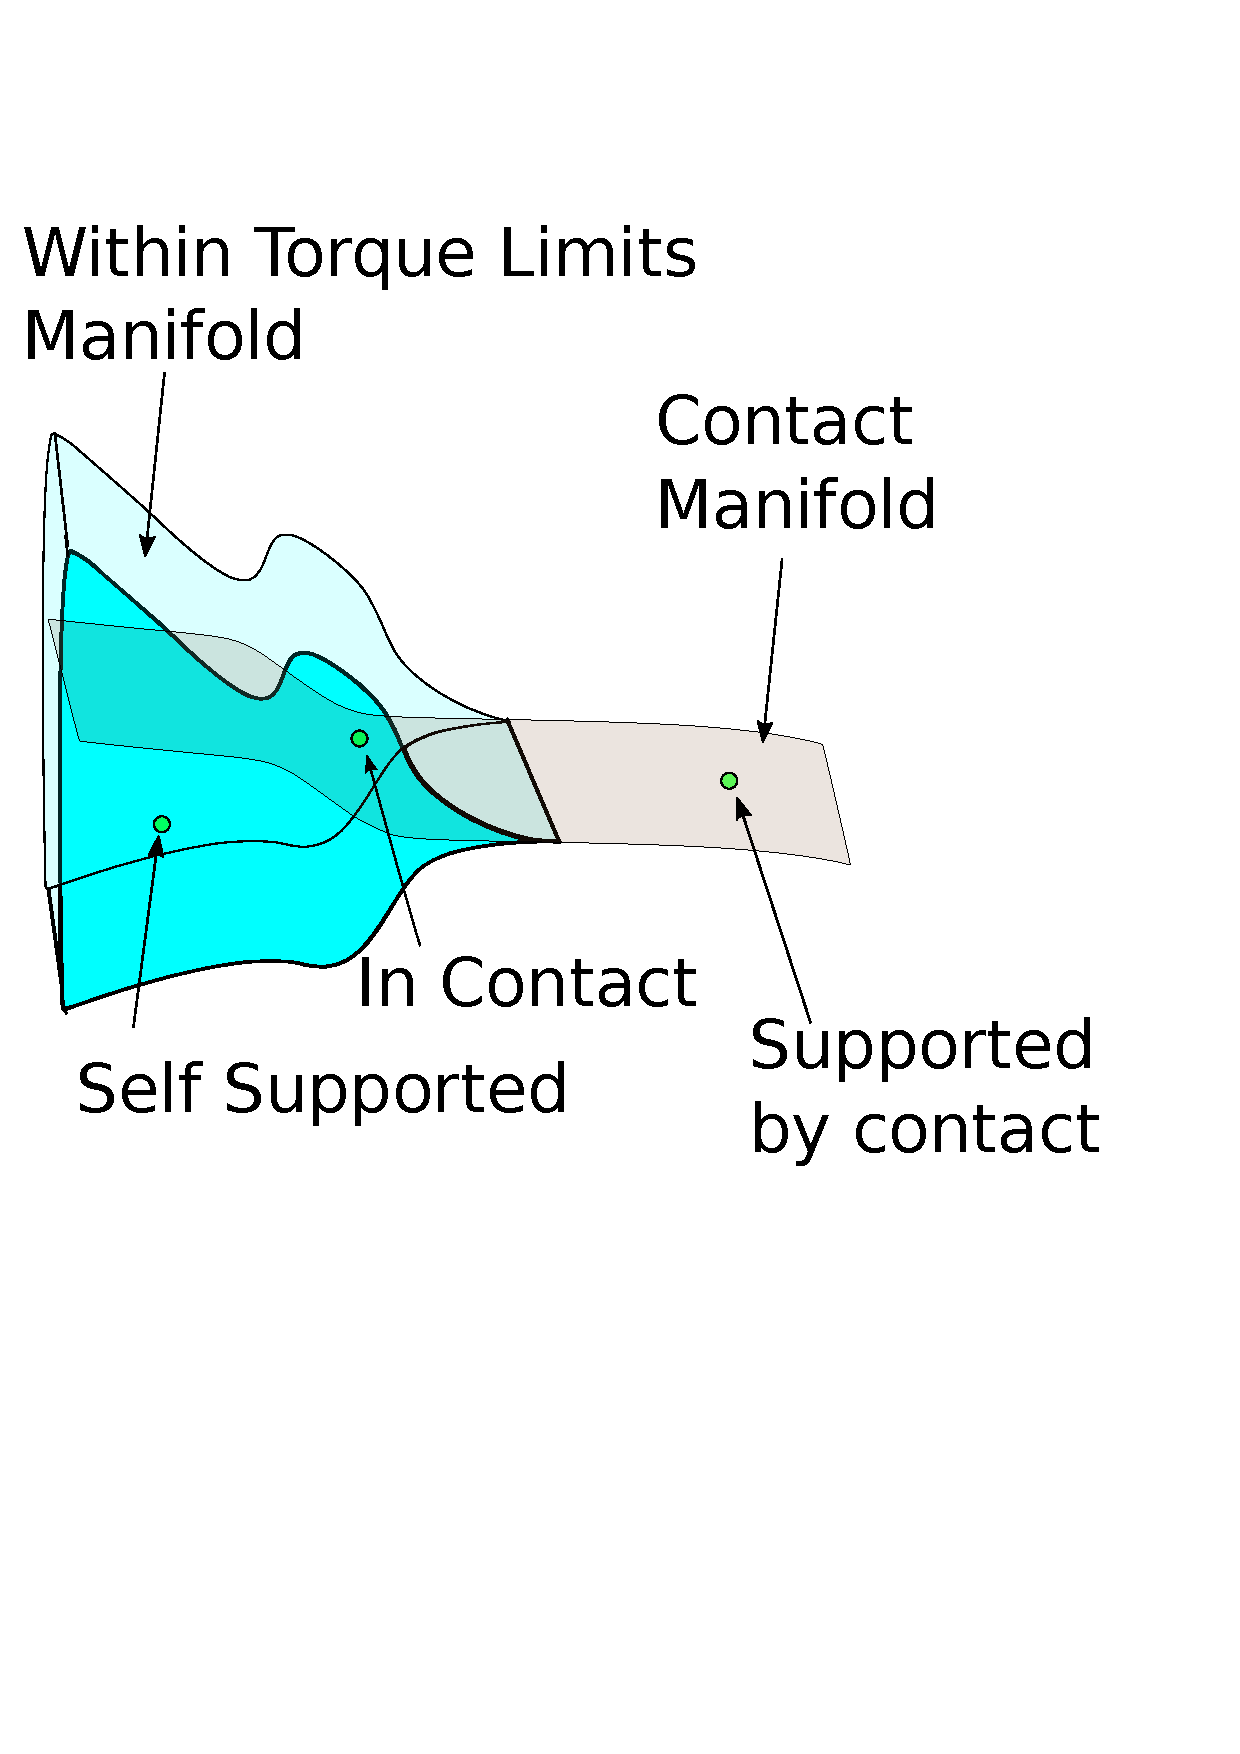
\includegraphics[width=.5\linewidth]{./Planning/thin_manifold.pdf}
  
  \caption{Illustration of valid configuration space for an arm potentially supported by contacts}
  \label{fig:thin_manifold}
\end{figure}

\subsection{Adaptation to Encourage Contacts}
This section describes the policyRRT algorithm, which by using a policy to guide the path extension is able to follow the contact manifold.

Given:
\begin{align}
    &X \in \mathbb{R}^d:     &&\text{d-dimensional configuration space}\\
    &X_{obs} \subset X:      &&\text{obstacles in the configuration space}\\
    &X_{free} = X \setminus X_{obs}:   &&\text{free space}\\
    &x_{start} \in X_{free}:  &&\text{starting configuration}\\
    &X_{goal} \subset X_{free}: &&\text{set of goal configurations}\\
    &policy: X \times X \rightarrow TX &&\text{Map from an initial and goal state to a motion}
\end{align}

The algorithm aims to find a path in $X_{free}$ from $x_{start}$ to $x_{goal} \in X_{goal}$.


\begin{algorithm}
\caption{$T=(V,E) \leftarrow$ policyRRT$(x_{start})$}\label{euclid}
\begin{algorithmic}[1]
\State $T \leftarrow$ InitTree($x_{start}$)
\While {GoalNotReached($T, X_{goal}$)}
\State $x_{rand} \in X \leftarrow$ Sample()
\State $x_{nearest} \leftarrow $ Nearest($T, x_{rand}$)
\State $T \leftarrow $ followPolicy$(x_{nearest}, x_{rand}, T$, extensionLimit)
\If {ExtensionSuccessful}
\State $T \leftarrow $ followPolicy$(x_{new}, x_{goal} \in X_{goal}, T, \infty)$
\EndIf
\EndWhile
\end{algorithmic}
\end{algorithm}

\begin{algorithm}
\caption{$T=(V,E) \leftarrow$ followPolicy$(x_{begin}, x_{end}, T$, iterLimit)}\label{euclid}
\begin{algorithmic}[1]
\State $T_{new} \leftarrow $ InitTree($x_{begin}$)
\State $x_{prev} \leftarrow x_{begin}$
\State $x_{new} \leftarrow $ policy($x_{prev}, x_{end}$)
\State $i \leftarrow 0$
\While{MovingTowardsGoal($x_{new}, T_{new}$) \textbf{and}
  Nearest($T, x_{new}$) == $x_{begin}$ \textbf{and}
  i $<$ iterLimit}
%% \algorithmicdo
\State $T_{new} \leftarrow $ AddNode($x_{new}, x_{prev}, T_{new}$)
\State $x_{prev} \leftarrow x_{new}$ 
\State $x_{new} \leftarrow $ policy($x_{prev}, x_{end}$)
\State $i \leftarrow i+1$
\EndWhile
\State $T \leftarrow $ AddTreeToTree($T_{new}, T, x_{begin}$)
\end{algorithmic}
\end{algorithm}

As motivation for this approach, in many environments it is relatively easy to compute a reactive policy that can make forwards progress towards a goal while avoiding collision with obstacles, such as a potential field approach, but such policies are prone to getting stuck in local minima.
PolicyRRT is a variant of RRT that seeks to combine the efficient, goal directed trajectory generation of reactive policies with the ability of RRT to find paths around local minima and dead ends.
PolicyRRT fundamentally behaves like a standard RRT by growing a tree by iteratively extending towards a randomly sampled configuration from the nearest point in a search tree $T$.
PolicyRRT uses the reactive policy to move towards the random sample, potentially enabling the planner to avoid collisions with obstacles during the extension.
When PolicyRRT is successful in extending towards the sample (does not collide with an obstacle and does not get stuck in a local minima) it then follows the policy to extend towards the goal.
To avoid oversampling regions associated with local minima, when PolicyRRT extends towards a point from some vertex $v \in T$ PolicyRRT halts extension when the trajectory leaves the Voronoi cell of $v$.
Extension is also halted once the policy ceases to make progress (reaches a local minima) or exceeds a maximum number of iterations.
%% (only when extending towards $x_{rand}$?)

%% PolicyRRT is beneficial when a policy that would yield a path all the way from $x_{start}$ and $x_{goal}$ is difficult to find but finding a policy that can make some progress while avoiding obstacles, but may get stuck in local minima is relatively easy.
%% An example of such a policy is a \textbf{potential field}: a cost function is constructed by placing attractors at the goals and repulsions at obstacles and the policy is to follow the gradient of this cost.
%% Potential fields are generally much simpler to compute than the minima-free navigation functions, but cannot be guaranteed to produce a path.
%% Augmenting the gradient descent policy with an RRT can help find paths out of any local minima.


\begin{figure}
  \centering
  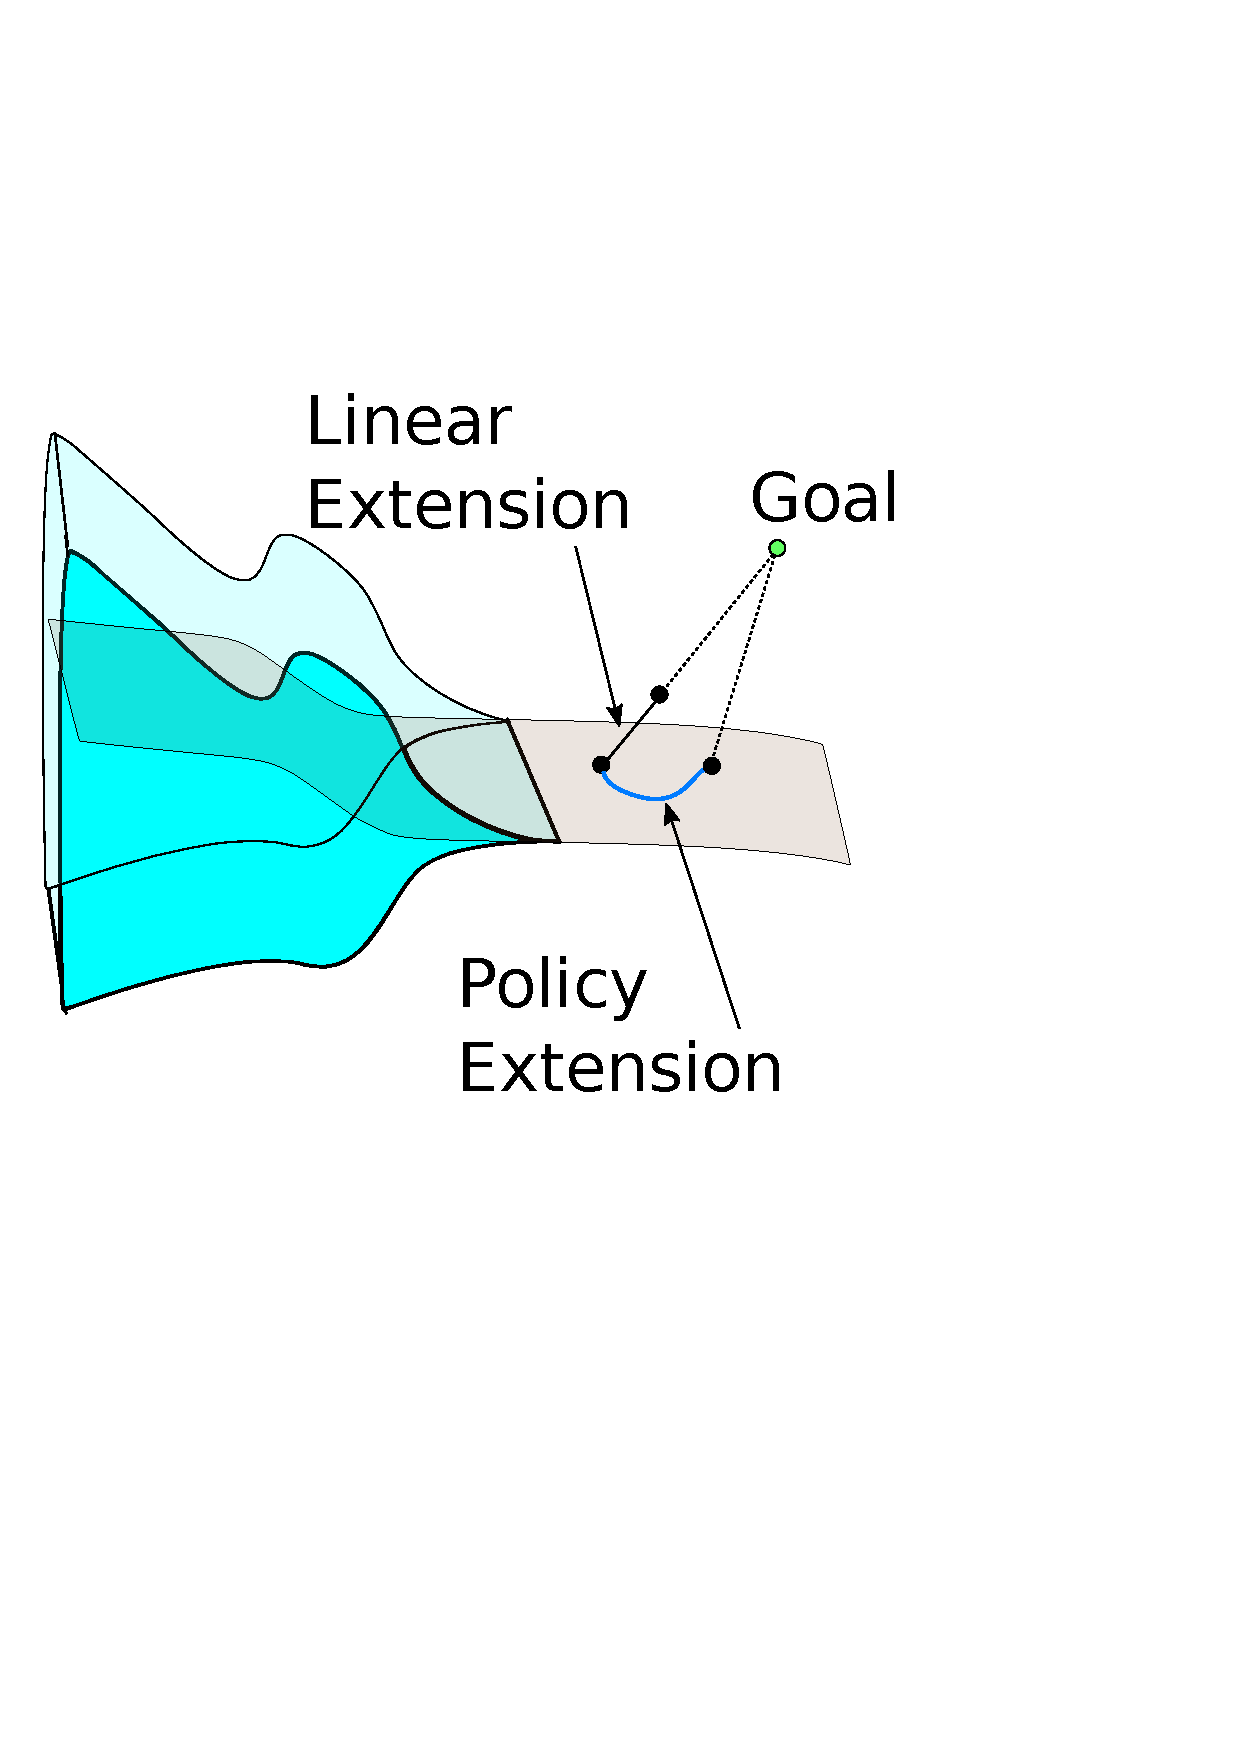
\includegraphics[width=.5\linewidth]{./Planning/extend.pdf}
  
  \caption{Illustration of Policy RRT extension on the contact manifold}
  \label{fig:extend}
\end{figure}

%% For configuration spaces where there is a thin contact manifold, The cost function constructed for trajectory optimiztaion, Eq. \ref{eq:cost}.


%% For the path planning problem with contact, the 

%% Similarly augmenting an RRT with a reactive policy can assist in navigating narrow passages.
%% Because the policy will naturally flow through corridors PolicyRRT no longer requires drawing samples inside the narrow corridor itself, as drawing a sample from the far side may suffice to draw the policy through the corridor.

The policy used in this algorithm should incorperate knowledge of the value of regions of configuration space to guide the extension function.
For the long arm planning with contact problem discussed in this chapter, the policy must direct the trajectory to maintain contact when necessary so the extension will be productive, but must allow the arm to break current and make new contacts for sufficiently exploration.
Fortunately, the gradient of the cost function use in the previous section for trajectory optimization (Eq. \ref{eq:cost}) has exactly these properties.
%% The 
%% By setting the goal configuration as the configuration randomly sampled by the RRT, the gradient of this cost function will direct the arm to explore towards this sample
Figure \ref{fig:extend} illustrates both the linear extension and this policy extension towards a randomly sampled goal configuration.
Leaving the contact manifold around these configurations causes large torques as the contact forces are removed, however because of the augmentation done in section \ref{sec:trajectory_optimization}, the gradient remains smooth so the policy pushes the arm back toward the support configurations.









\section{Experiments}
\subsection{Comparison to non-contact plans}
\begin{table}
\centering
%% \vspace{3em}
\resizebox{\textwidth}{!}{\begin{tabular}{| l | c | c | c | c |}
    \hline
    & 0m & 0.5m & 1m & 1.3m
    %% & Measurement    & Init. Position & Init. Angular & Final Position & Final Angular & Average \\
    %% & Error (cm)    & Uncertainty (cm) & Uncertainty (rad) & Error (cm) & Error (rad) & Computation 
    \\
    \hline
    Optimization without contacts: planned & 6.91 (0.81) & 7.12 (0.74) & 5.87 (0.89) & 7.74 (1.14)\\
    \hline
    Optimization without contacts: actual & 4.47 (0.58) & 4.34 (0.65) & $\dagger$ & $\dagger$\\
    \rowcolor[gray]{.8}
    \hline
    Optimization with contacts: planned  & 0.01 (0.00)& 0.01 (0.00) & 0.05 (0.00) & 0.03 (0.00)\\
    \rowcolor[gray]{.8}    
    \hline
    Optimization with contacts: actual & 2.40 (0.46) & 2.10 (0.61) & 2.46 (0.56) & 2.03 (0.55)\\
    \hline
    RRT without contacts: planned & 4.12 (0.91) & 4.87 (0.54) & $\dagger$ & $\dagger$\\
    \hline
    RRT without contacts: actual & 5.53 (0.48) & 4.81 (0.58) & $\dagger$ & $\dagger$\\
    \hline
  \end{tabular}}
  \captionof{table}{Joint torques for a long 11-DOF robotic arm following trajectories generated by different planners to a goal point at specified horizontal distances from the robot base. Values are reported as the \boxed{\text{max (avg)}} torques over all links over all time steps in newton-meters. $\dagger$ indicates the failure to plan or execute a trajectory.}
  \label{table:non_contact_comparison}
\end{table}

\begin{figure}
  \centering
  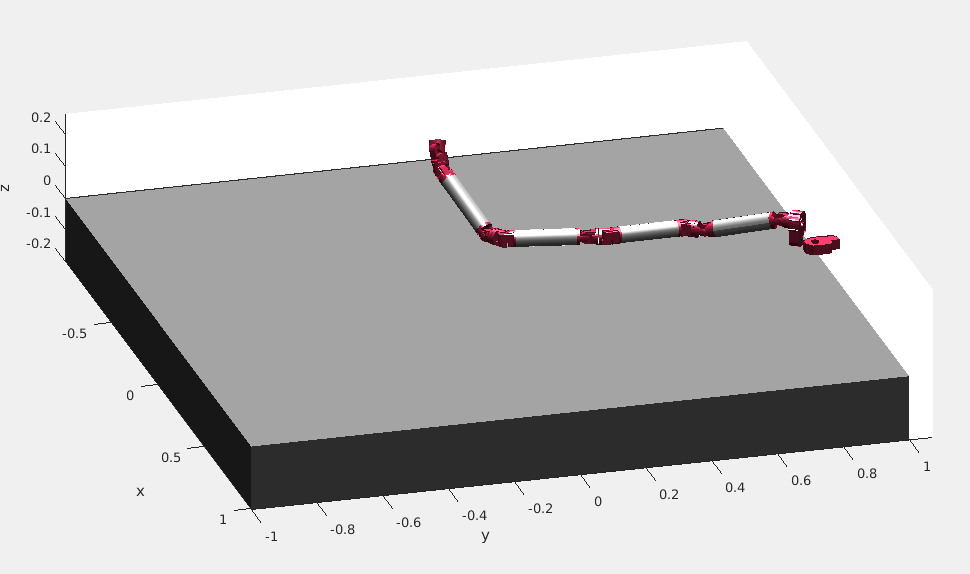
\includegraphics[width=.7\linewidth]{./Planning/flat_ground_arm.png}
  \caption{Final state of the ``optimization with contacts'' plan for the snake-like arm reaching far from the base, supported by the environment}
  \label{fig:flat_ground_arm}
\end{figure}

Experiments were preformed to demonstrate the benefits of planning with contact.
Three algorithms were used to generate plans: the naive trajectory optimization that is not able to discover contacts, the smooth contact trajectory optimization as described in section \ref{sec:trajectory_optimization},  and an RRT. 
Plans were generated for an approximately 1.5 meter long 11-DOF arm in a world with a flat floor.
Each joint had a maximum torque limit of 5 Nm.
The different goal positions included moving the end effector directly above, 0.5, 1, and 1.3 meters from the base link.
Figure \ref{fig:flat_ground_arm} visualizes the simulated arm in this environment.

Table \ref{table:non_contact_comparison} displays the maximum and average torques experienced by the links.
Both in simulation and on the physical robot it is clear allowing contacts can significantly reduce the joint torque.
The joints can support the arm when cantilevered out 0m and 0.5m, and both naive optimization and the RRT find paths that are feasible on the robot, yet the joint torques are significantly reduced when supporting contacts are found.
The joints are unable to support the arm when cantilevered 1m and 1.3m from the base, causing the RRT to never find a feasible path. Because the implementation of the naive optimization uses soft limits on joint torque, a path is found in simulation but this trajectory fails to execute properly on the physical robot.

By using contacts the trajectory optimization using an augmented dynamics model is able to plan paths for each of these goal points.
Contacts nearly eliminate joint torques in simulation.
In practice the joints torques remain decently large due to friction in the joints and other losses, as well as inaccuracies in the environment and robot model, causing contacts to occur at slightly different joint angles than expected.
However, because the robot uses compliant actuators it is acceptable for contact to occur slightly earlier or later than expected.




\subsection{Planning in an Airplane Wing}
\begin{figure}
  \centering
  \begin{subfigure}[b]{.48\linewidth}
    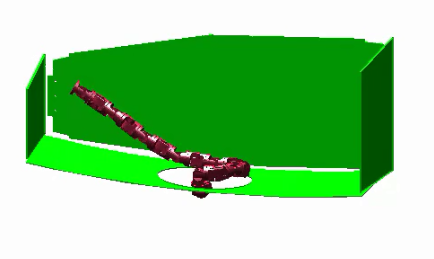
\includegraphics[width=\linewidth]{./Planning/simulated_snake_in_wing.png}
  \end{subfigure}
  \begin{subfigure}[b]{.48\linewidth}
    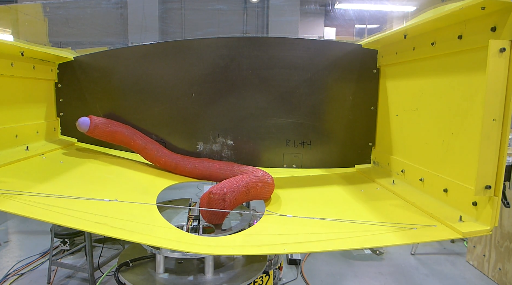
\includegraphics[width=\linewidth]{./Planning/real_snake_in_wing.png}
  \end{subfigure}
  
  \caption{Simulated (left) and actual (right) snake arm robots executing motions planned in a model of an airplane wing section}
  \label{fig:snake_in_wing}
\end{figure}

Trajectories were generated for a 16-DOF snake robot arm in a model of a wing section by combining the approaches shown above.
The initial configuration and goal position for the end effector were chosen manually and contained goal positions at the corners of the available volume so that the arm must maintain contact for support.

First, the policyRRT of section \ref{sec:sample_planning} was used to generate a trajectory a for the arm to a goal position while avoiding collisions between the robot and the wing, however ignoring the torque limits of the joints.
This trajectory was used as an initialization for the trajectory optimization approach of section \ref{sec:trajectory_optimization}




%% \subsection{Simulation and Robot Model}
%% \subsection{Robot Snakes on a Plane}

\end{document}
